
%----------------------------------------------------------------------------------------
%	Lecture 11
%----------------------------------------------------------------------------------------

\chapter{Double Integrals}

\bigbreak

In single variable calculus, \ilds{\int_a^b f(x) dx = } area of the curve under the curve.

For functions with two variables, you can try to find the volume below the graph $z = f(x, y)$ and that is what call the double integral of that function.

For double integral, we need to choose a region, R, in the XY-plane to integrate over and we'll try to measure the volume under the curve over that region.

$$ \iint_{R} f(x, y) dA $$

In sinlge variable calculus, we divided the interval into many different pieces and added the area of all the pieces to obtain the area.
Here, we will divide the region R into small rectangles with $\Delta A$ as the area of the $i^{th}$ rectangle at position $(x_i, y_i)$. Thus, we approximate the volume by

$$  \sum_i f(x_i, y_i) \Delta A $$

Finally, we take the limit as the area of the rectangle goes to $0$.

$$ \lim_{\Delta A \to 0} \sum_i f(x_i, y_i) \Delta A = \iint_R f(x, y) dA $$

When taking derivative of multivariate function, we were using slices of places to calculate derivative with respect to one variable.
We can do the same here. Let's take a slice $x = x_0$ of width $dx$. 
In this slice, we will get a single variable integral which will give us the area of the cross section. 
So the volume of these slice will be $(area) * dx$. 

\begin{figure}[ht!]
    \centering
    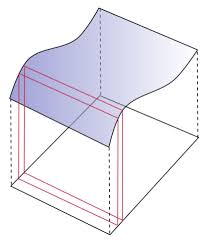
\includegraphics[scale=0.7]{./images/lecture_11_figure_1.jpeg}
    \caption{Slice of the volume over a region}
\end{figure}

To find the volume, we can add all the volumes of these slices.
As the width of the slices tend to zero, the total sum approaches the volume.

Let the area of the slice be $S(x)$. So, $$ Volume =  \int_{x_{min}}^{x_{max}} S(x) dx $$

Now you can compute the area as $$ S(x) = \int_{y_{min}(x)}^{y_{max}(x)} f(x, y) dx $$ where $x$ is constant as we are taking the slice $x = x_0$.

Here, the range of integration of $y$ is a function of $x$ because the slice will have different widths everywhere.

For example, we we take a circular region and take the slice $x = x_0$, the range of $y$ changes depending upon how far $x = x_0$ is from the center of the circle.

Thus, finally, we get,
$$ \iint_R f(x, y) dA = \int_{x_{min}}^{x_{max}} \left[ \int_{y_{min}(x)}^{y_{max}(x)} f(x, y) dy  \right] dx $$

This is called an iterated integral. Here the values of $x_{min}$ and $x_{max}$ will be constants.
On the otherhand, $y_{min}$ and $y_{max}$ will depend on the outer variable $x$.


{\bf Example : } $z = 1 - x^2 - y^2$ for $0 <= x <= 1$ and $0 <= y <= 1$.

$$Volume = \int_0^1 \int_0^1 (1 - x^2 - y^2) dy dx$$

Let's do the inner integral first.

$$ \int_0^1 (1-x^2-y^2) dy 
    = \left[ y - x^2y - \frac{y^3}{3} \right]_0^1 
    = \left( 1 - x^2 - \frac{1}{3} \right) - 0 = \frac{2}{3} - x^2
$$

Now, for the volume,

$$ Volume = \int_0^1 \frac{2}{3} - x^2 dx 
    = \left[ \frac{2x}{3} - \frac{x^3}{3} \right]_0^1 
    = \left( \frac{2}{3} - \frac{1}{3} \right) - 0 = \frac{1}{3}
$$


{\bf Note : }
Earlier we took the slices in the x-direction but we can also do the same for y-direction. 
In theory, the order of the integration does not matter but in practice, the difficulty of the order of integration might vary depending on the region.
So, we have to be careful in setting up the order of the integration because one way might be much harder than the other.

\pagebreak

{\bf Example : }
Let's say we wanted to intergrate $z = 1 - x^2 - y^2$ over the area in the first quadrant where $z > 0$.
So $x >= 0$, $y >= 0$ and $x^2 + y^2 <= 1$. This is the same integral as above but the bounds are different.

For a given $x$, the range of $y$ is $y = 0$ to $y = \sqrt{1 - x^2}$. 
Here, we take only the positive square root as $y >= 0$.

Now the final range of $x$ will be $x = 0$ to $x = 1$ as that is the rightmost point in our region.

\begin{figure}[ht!]
    \centering
    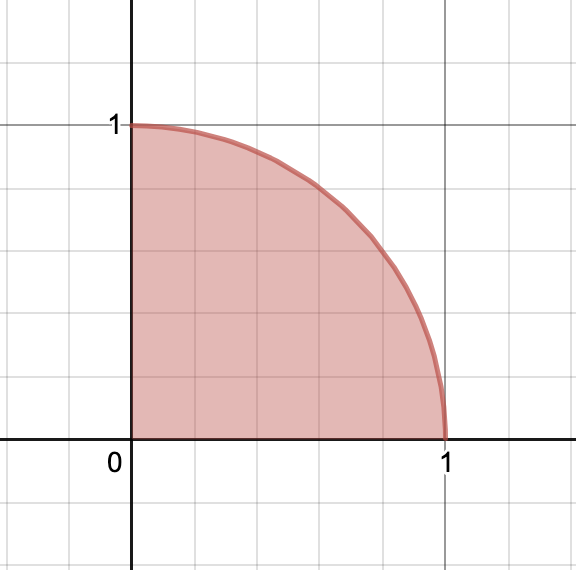
\includegraphics[scale=0.5]{./images/lecture_11_figure_2.png}
    \caption{The region $x^2 + y^2 <= 1$ in the first quadrant}
\end{figure}

So the final volume will be,

$$ \iint_R (1-x^2-y^2) dA = \int_0^1 \int_0^{\sqrt{1-x^2}} (1-x^2-y^2) dy dx $$

Solving the inner integral, 

$$ \int_0^{\sqrt{1-x^2}} (1-x^2-y^2) dy 
    = \left[ y - x^2y - \frac{y^3}{3} \right]_0^{\sqrt{1-x^2}}
    = \left( \sqrt{1-x^2} - x^2\sqrt{1-x^2} - \frac{(\sqrt{1-x^2})^3}{3} \right) - 0
    = \frac{2}{3} (\sqrt{1-x^2})^3
$$ 

$$
Volume = \int_0^1 \frac{2}{3} (1-x^2)^{3/2} dx 
$$

To solve this, let's so a trig substitution, $x = \sin \theta$ so $\sqrt{1-x^2} = \cos \theta$ and $dx = \cos \theta d\theta$.

$$
Volume = \int_0^{\frac{\pi}{2}} \frac{2}{3} \cos^3(\theta) \cos(\theta) d\theta
$$

You can solve this, using the double angle formula $\cos(2\theta) = 2\cos^2(\theta) - 1$.
If you solve this, then you'll get \ilds{ Volume = \frac{\pi}{8} }

This will be easier in polar coordinates.


\subsection*{Exchanging the order of integrals}

You can change the order of the integrals and you'll get the same volume.
Let's take an example.

$$ \int_0^1 \int_x^{\sqrt{x}} \frac{e^y}{y} dy  dx $$

There is no way to integrete \ilds{\frac{e^y}{y}} so we'll have to change the order of integration.
For that we'll need to understand the region.

\begin{figure}[ht!]
    \centering
    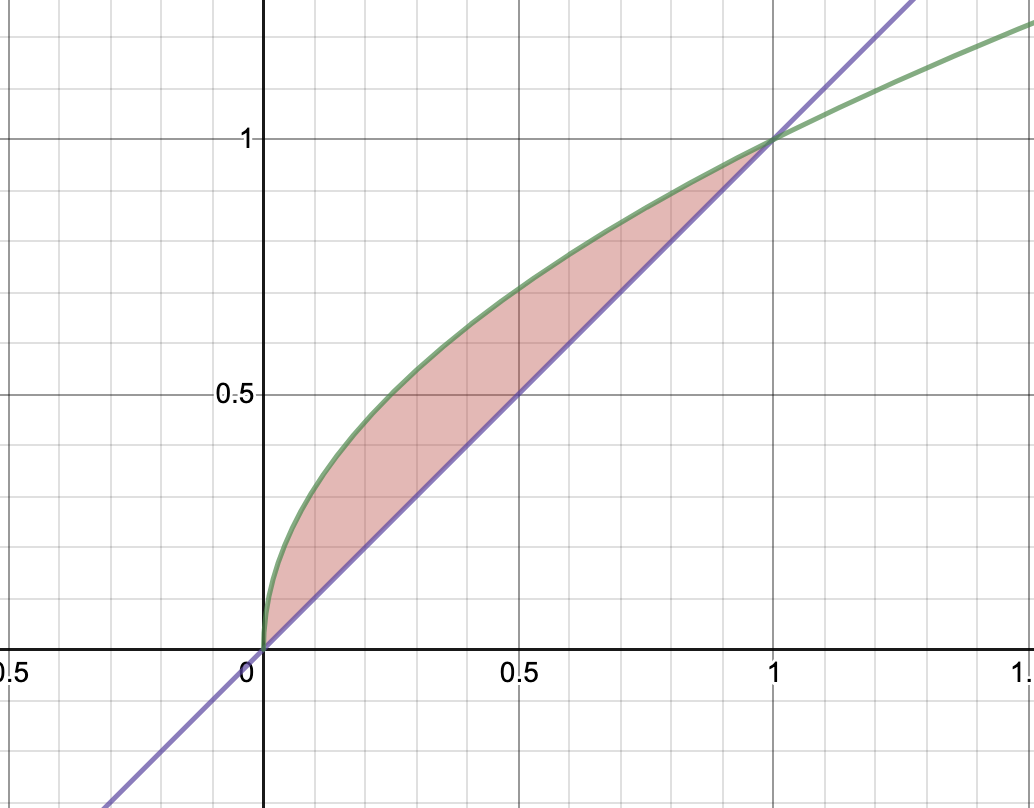
\includegraphics[scale=0.5]{./images/lecture_11_figure_3.png}
    \caption{The region for above example}
\end{figure}

Now we can do it the otherway around. 
If we fix a $y$ then the range for $x$ is $x = y^2$ to $x = y$.
The range of $y$ is $y = 0$ to $y = 1$.

\begin{align*}
\iint \frac{e^y}{y} dA  
        & = \int_0^1 \int_{y^2}^{y} \frac{e^y}{y} dx dy \\
        & = \int_0^1 \left[ \frac{e^y}{y} x \right]_{y^2}^y dy \\
        & = \int_0^1 \left( e^y - e^y y \right) dy \\
        & = \left[ 2e^y - ye^y \right]_0^1 = e - 2
\end{align*}